\documentclass{article}
\usepackage[utf8]{inputenc}

\title{Homework No.8}
\author{Osamu Katagiri-Tanaka : A01212611}
\date{\today}

% import math symbols
\usepackage{amsmath, esint}
\usepackage{cancel}

% multiline equations
\usepackage{breqn}

% import code snippets
\usepackage{listings}
\usepackage{xcolor}
\definecolor{codegreen}{rgb}{0,0.6,0}
\definecolor{codegray}{rgb}{0.5,0.5,0.5}
\definecolor{codepurple}{rgb}{0.58,0,0.82}
\definecolor{backcolour}{rgb}{0.99,0.99,0.96}
\lstdefinestyle{mystyle}{
  backgroundcolor   = \color{backcolour},
  commentstyle      = \color{codegreen},
  keywordstyle      = \color{magenta},
  numberstyle       = \tiny\color{codegray},
  stringstyle       = \color{codepurple},
  basicstyle        = \ttfamily\small,
  breakatwhitespace = false,
  breaklines        = true,
  captionpos        = b,
  keepspaces        = true,
  numbers           = left,
  numbersep         = 2pt,
  showspaces        = false,
  showstringspaces  = false,
  showtabs          = false,
  tabsize           = 2,
  aboveskip         = 0.1em,
  belowskip         = 0.1em
}
\lstset{style=mystyle}

% import hyperlinks
\usepackage{hyperref}
\hypersetup{
  colorlinks = true,
  linkcolor  = red,
  filecolor  = red,
  citecolor  = red,
  urlcolor   = red
}

% import continuous lists
\usepackage{enumitem}

% format margins and paper size
\usepackage{geometry}
\geometry{
	paper         = a4paper, % Change to letterpaper for US letter
	inner         = 2.5cm,   % Inner margin
	outer         = 2.5cm,   % Outer margin
	bindingoffset = 0.5cm,   % Binding offset
	top           = 1.5cm,   % Top margin
	bottom        = 1.5cm    % Bottom margin
}

% import figure handler
\usepackage{graphicx}

% import references handler
\usepackage[
  style     = ieee,         % references format style
  backend   = biber,        % choose the processing program
  natbib    = true,         % enable additional reference formats
  citestyle = numeric-comp, % enable multiple citations
  sortcites = true,         % sort references in multiple citations
  sorting   = nyt           % sort the reference table
]{biblatex}
\addbibresource{references.bib}

% Note that ‘d’ in the differential is conventionally set in roman.
\newcommand{\ud}{\,\mathrm{d}}

% Paragraph spacing
\setlength{\parskip}{0.2cm}           % spacing between paragraphs
\renewcommand{\baselinestretch}{1.25} % spacing between lines

\begin{document}

\maketitle

\subsection*{Simulate the cooling of apple/avocado considering, convection and radiation.}

\begin{figure}[h!]
	\centering	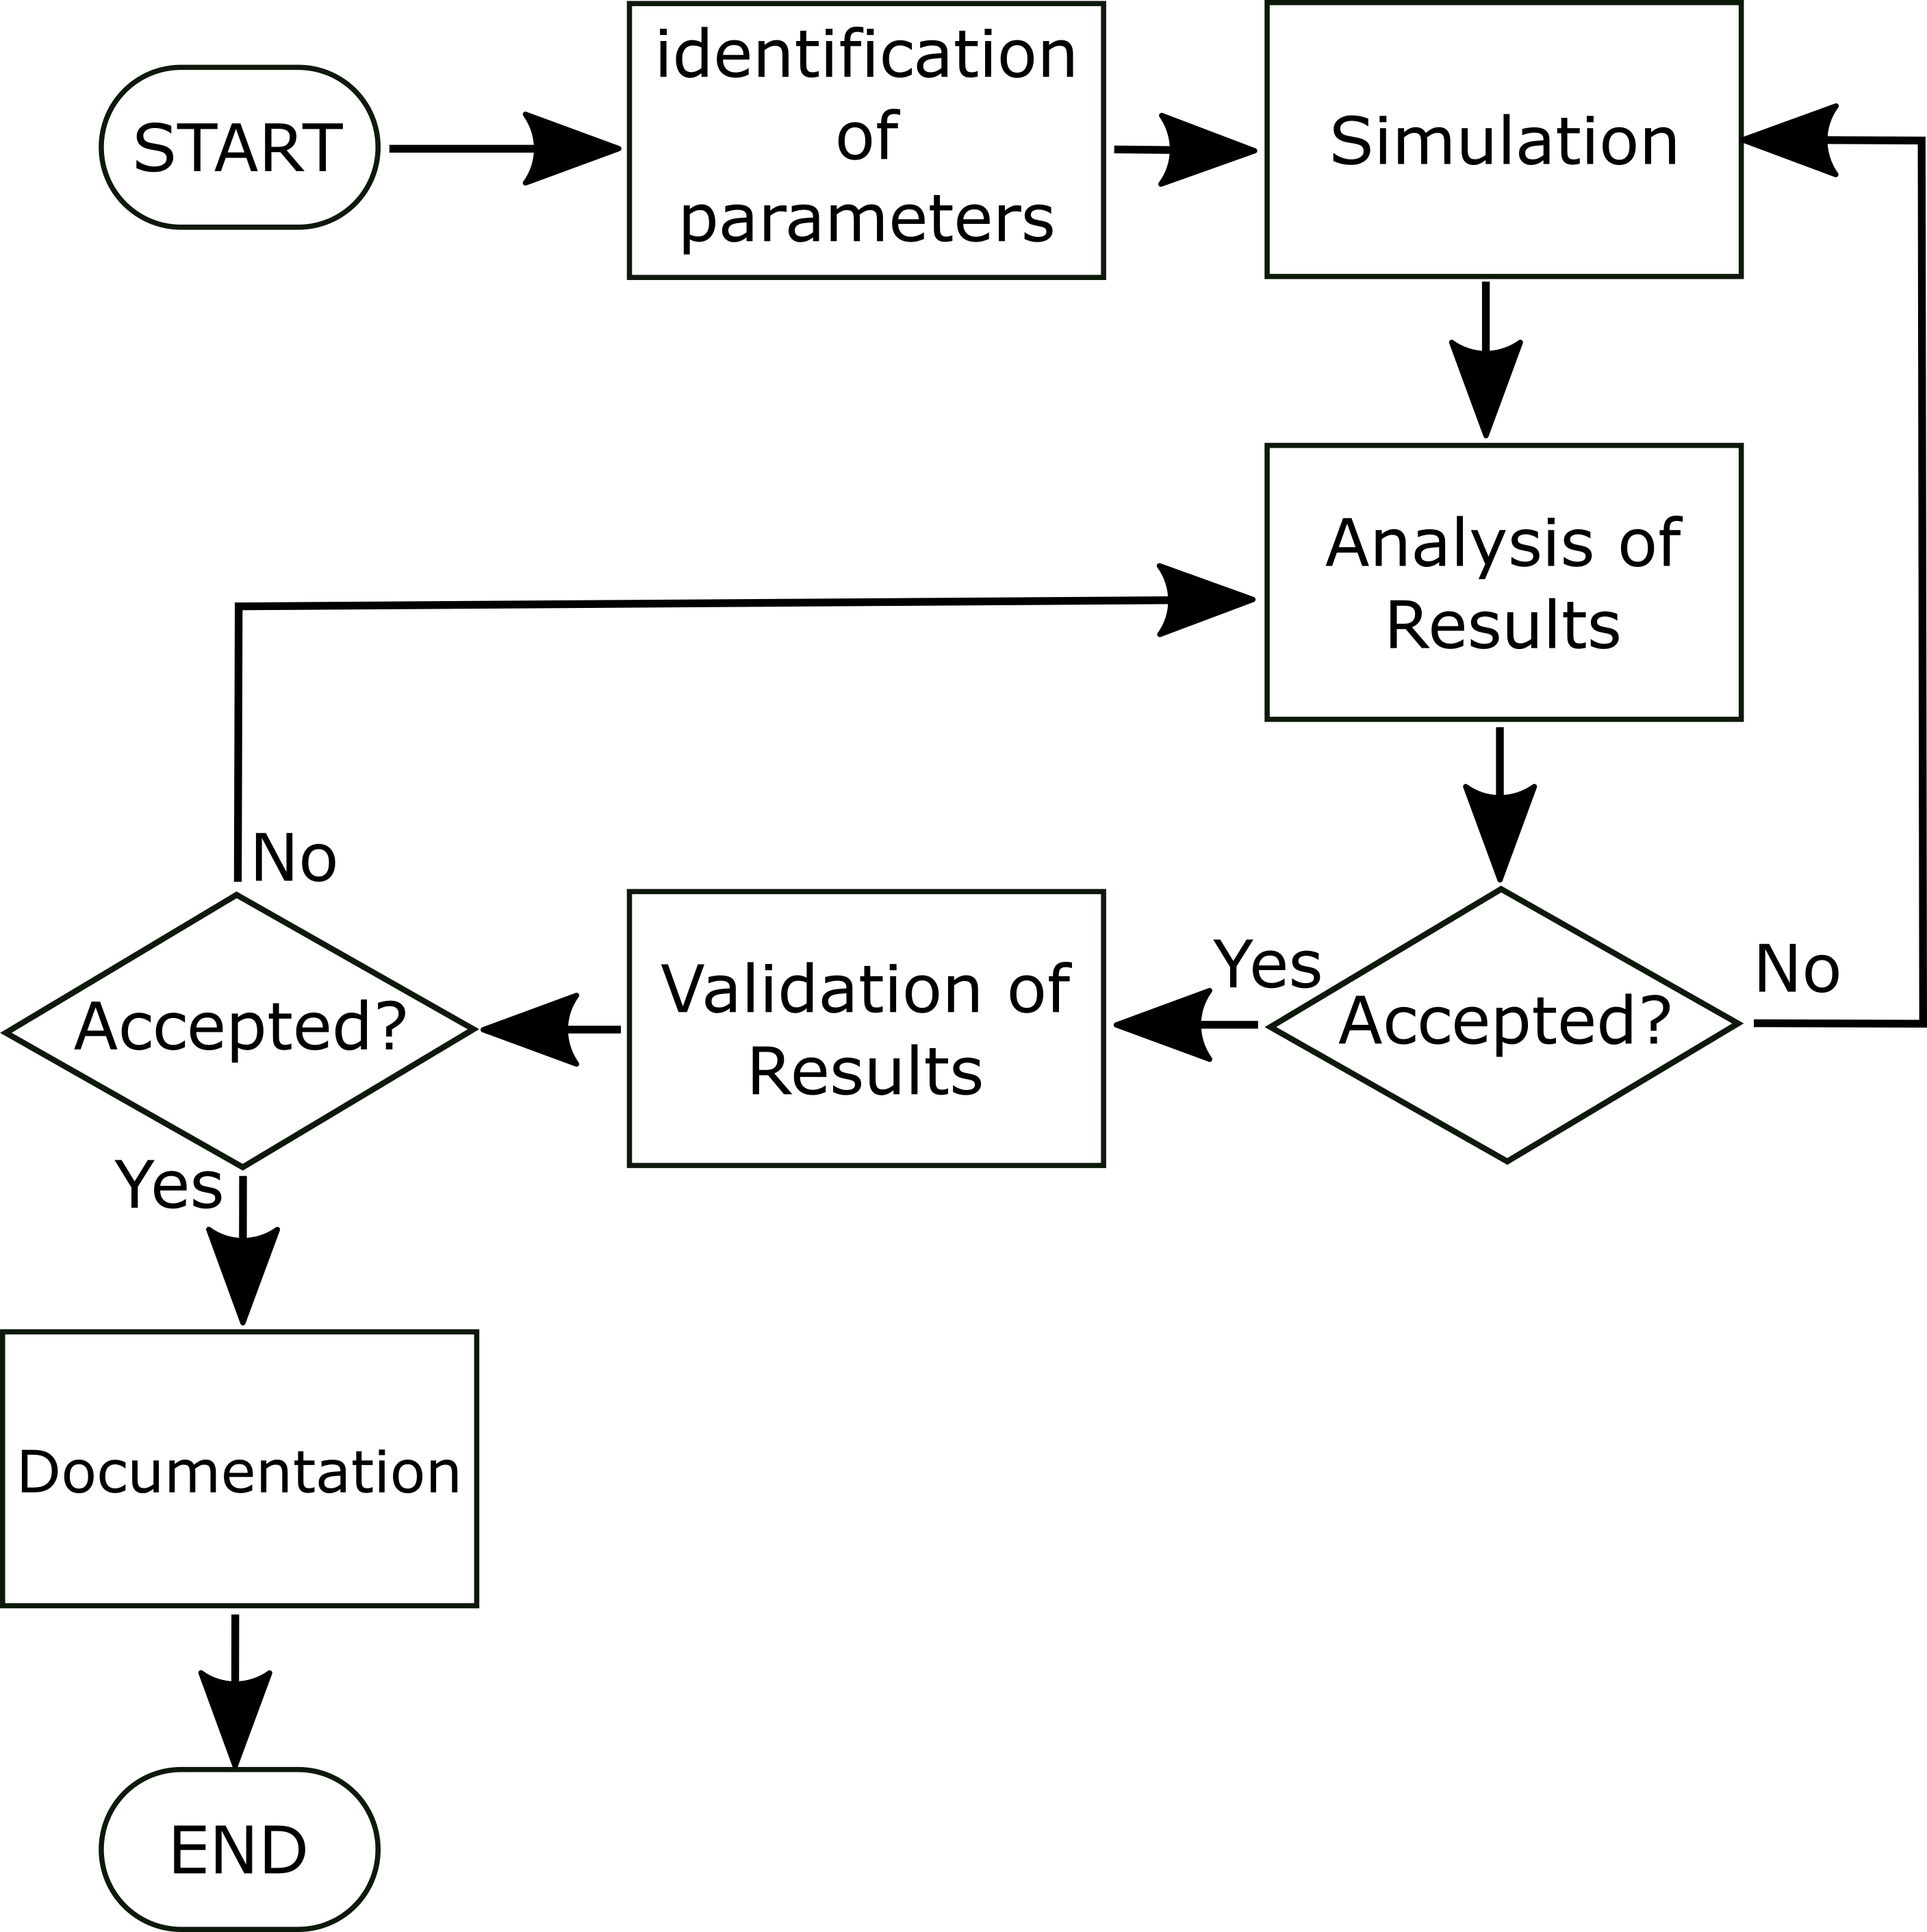
\includegraphics[width=0.40\textwidth]{./Flowchart.png}
	\caption{Process Flowchart of CFD simulation}
	\label{img:Flowchart}
\end{figure}

Simulation is done under the following conditions:
\begin{itemize}
\item Initial temperature of the fruit $25^{\circ} \textrm{C}$. (Fruit is assumed to be a spherical apple)
\item surroundings temperature $-10^{\circ} \textrm{C}$
\item Air must be stangant or moving at velocity not higher than $2 \textrm{m}/\textrm{s}$. ($v_{air} = 0 \textrm{m}/\textrm{s}$ is assumed)
\item The methabolic/respiration rate of the fruit must be $40 \textrm{mW} / \textrm{kg}$
\end{itemize}

Ansys - Transient Thermal is used to simulate the cooling of an apple through convection and radiation. As shown in Figure \ref{img:Flowchart}, the cooling effect is first simulated and then validated through an analytic solution. Results compare the effect of the object's shape as a "spherical-apple" and a "cylindrical-apple" are analyzed.

As the surface of the object is subjected to both convection and radiation, let's do a energy balance on the control volume, assuming the temperature of the sphere is uniform:

\begin{dmath}
\left( \begin{matrix}
\textrm{Heat in}\\
\textrm{via}\\
\textrm{Convection}
\end{matrix} \right) +
\left( \begin{matrix}
\textrm{Heat in}\\
\textrm{via}\\
\textrm{Radiation}
\end{matrix} \right) = 0
\end{dmath}

\begin{dmath}
\frac{d}{d t} (\rho V c T) = -(\dot{q}_{conv} + \dot{q}_{rad})
\end{dmath}

\begin{dmath}
\frac{d T}{d t} = - \frac{A}{\rho V c} \left[ h (T - T_{\infty}) + \varepsilon \sigma (T^4 - {T_{surr}}^4) \right]
\end{dmath}

\begin{figure}[h!]
	\centering
	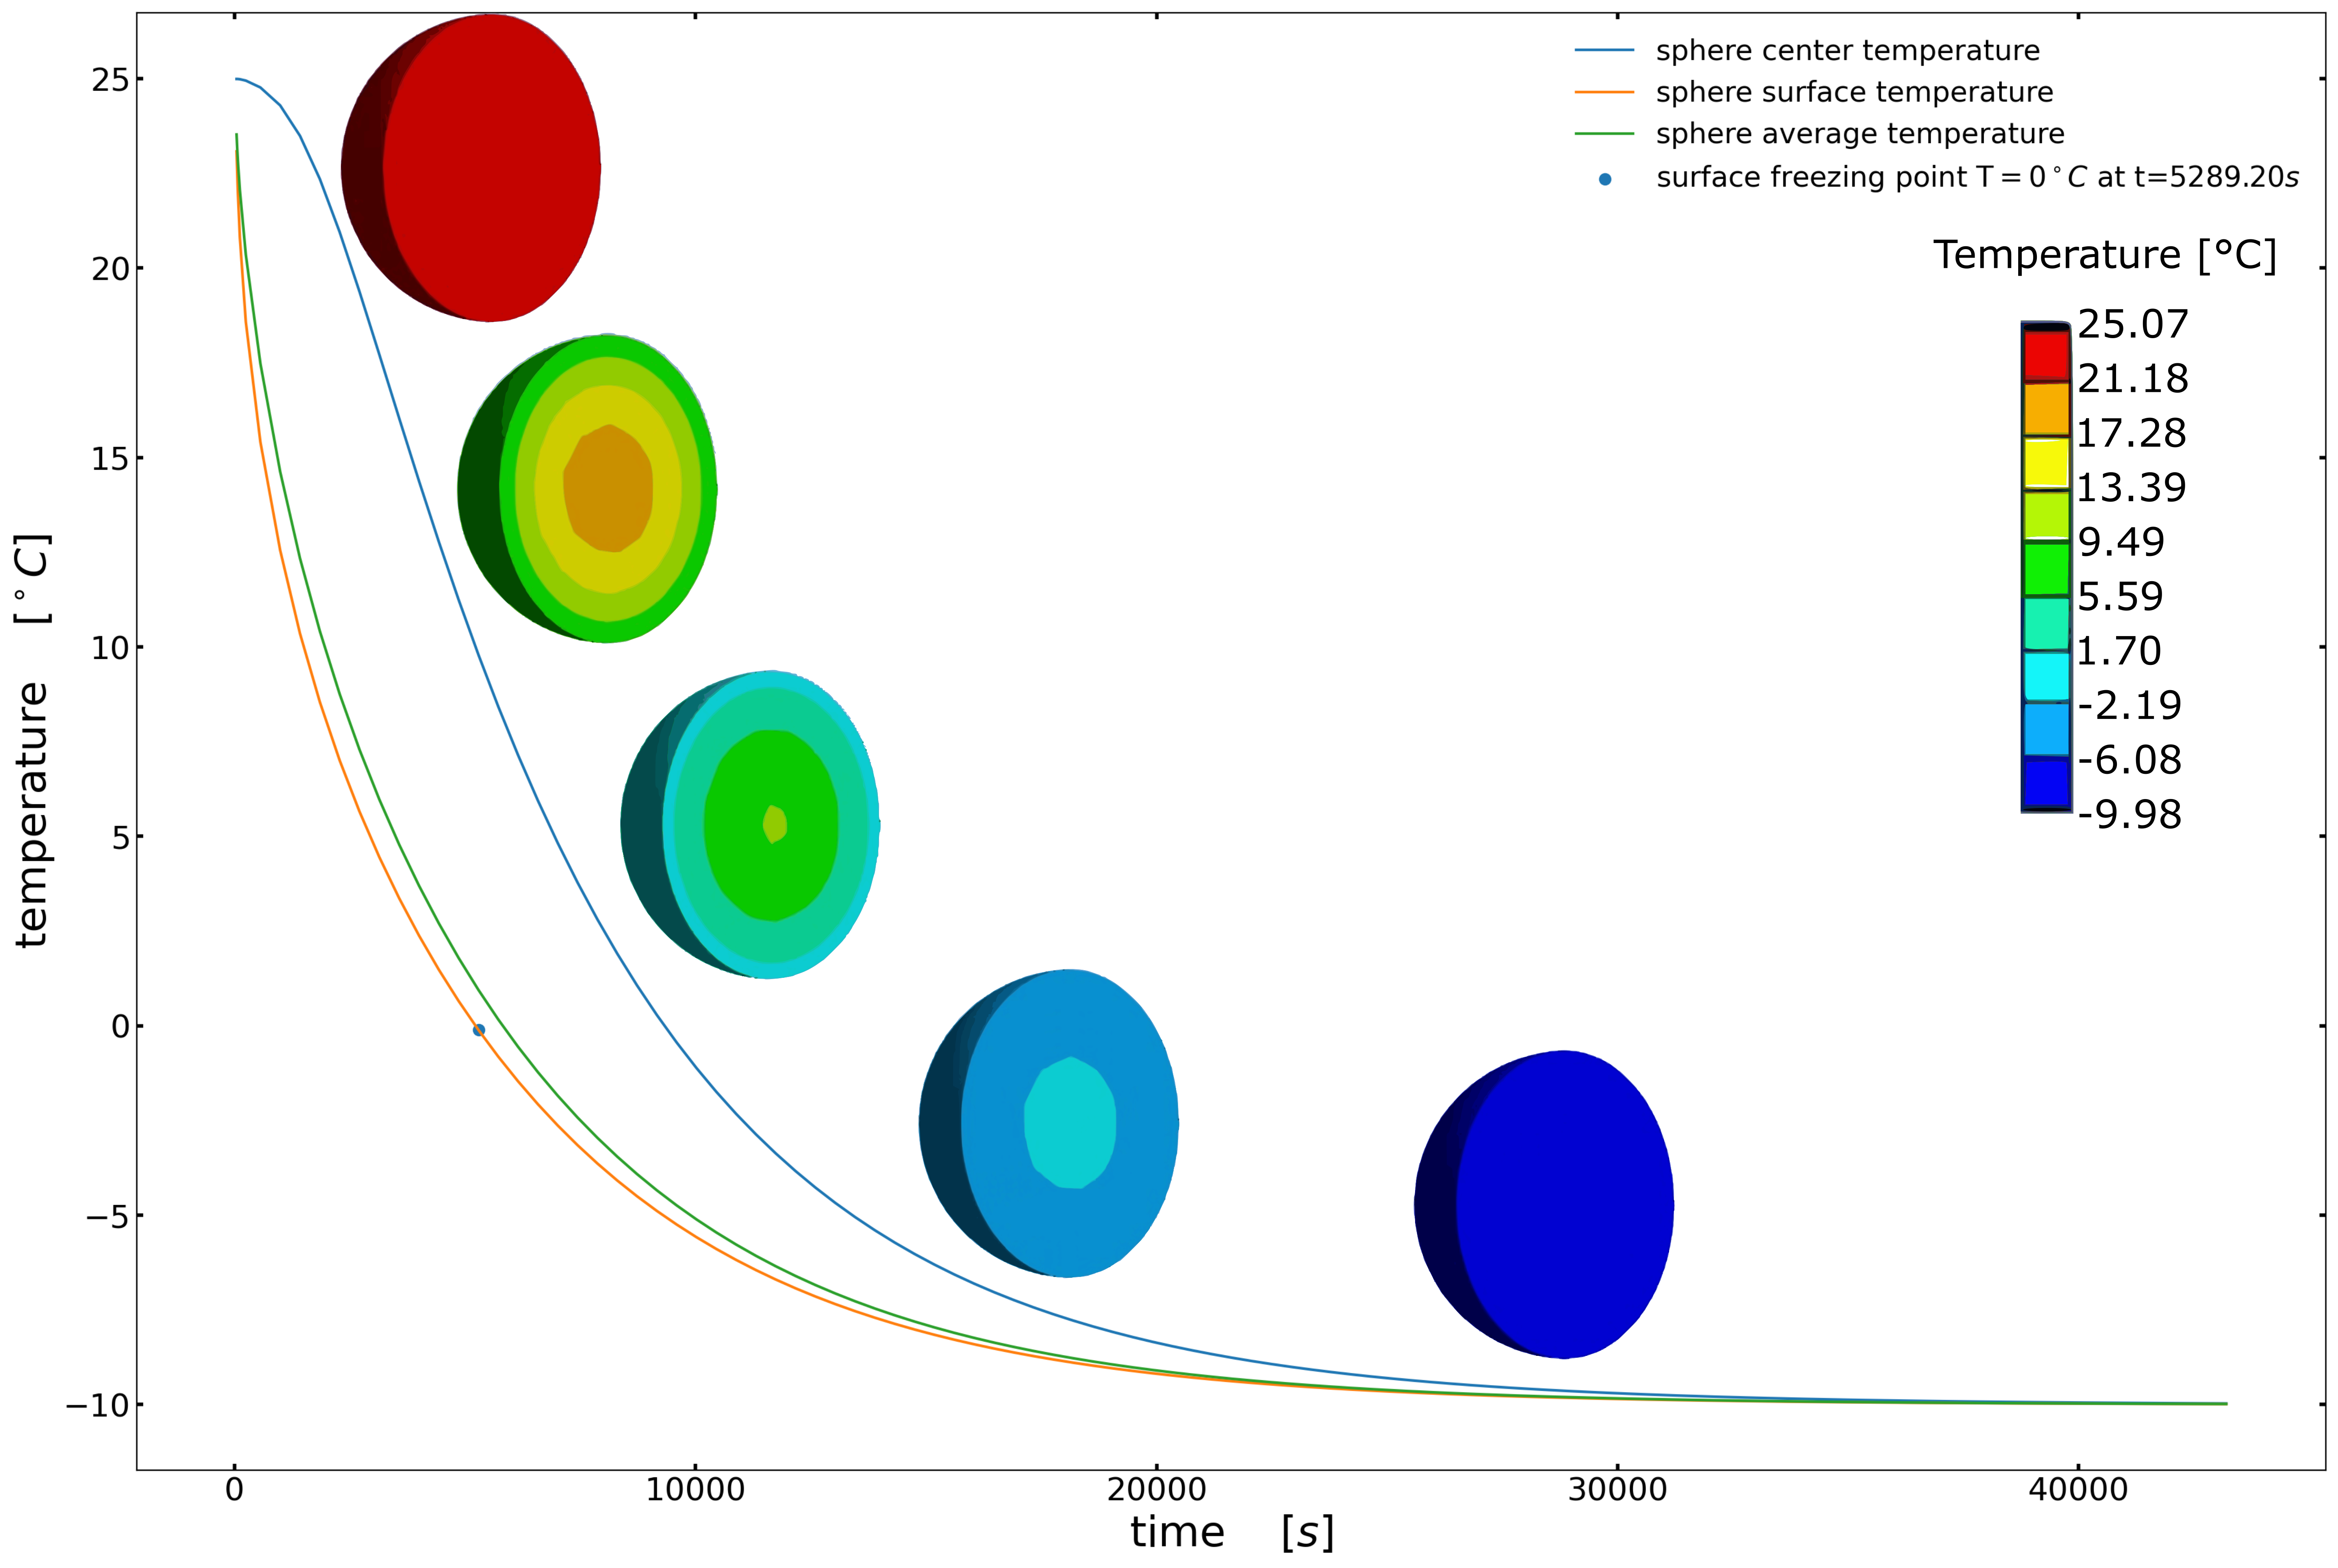
\includegraphics[width=1.00\textwidth]{./sphereTemps.png}
	\caption{Visualization of a Velocity Field}
	\label{img:sphereTemps}
\end{figure}

\begin{figure}[h!]
	\centering
	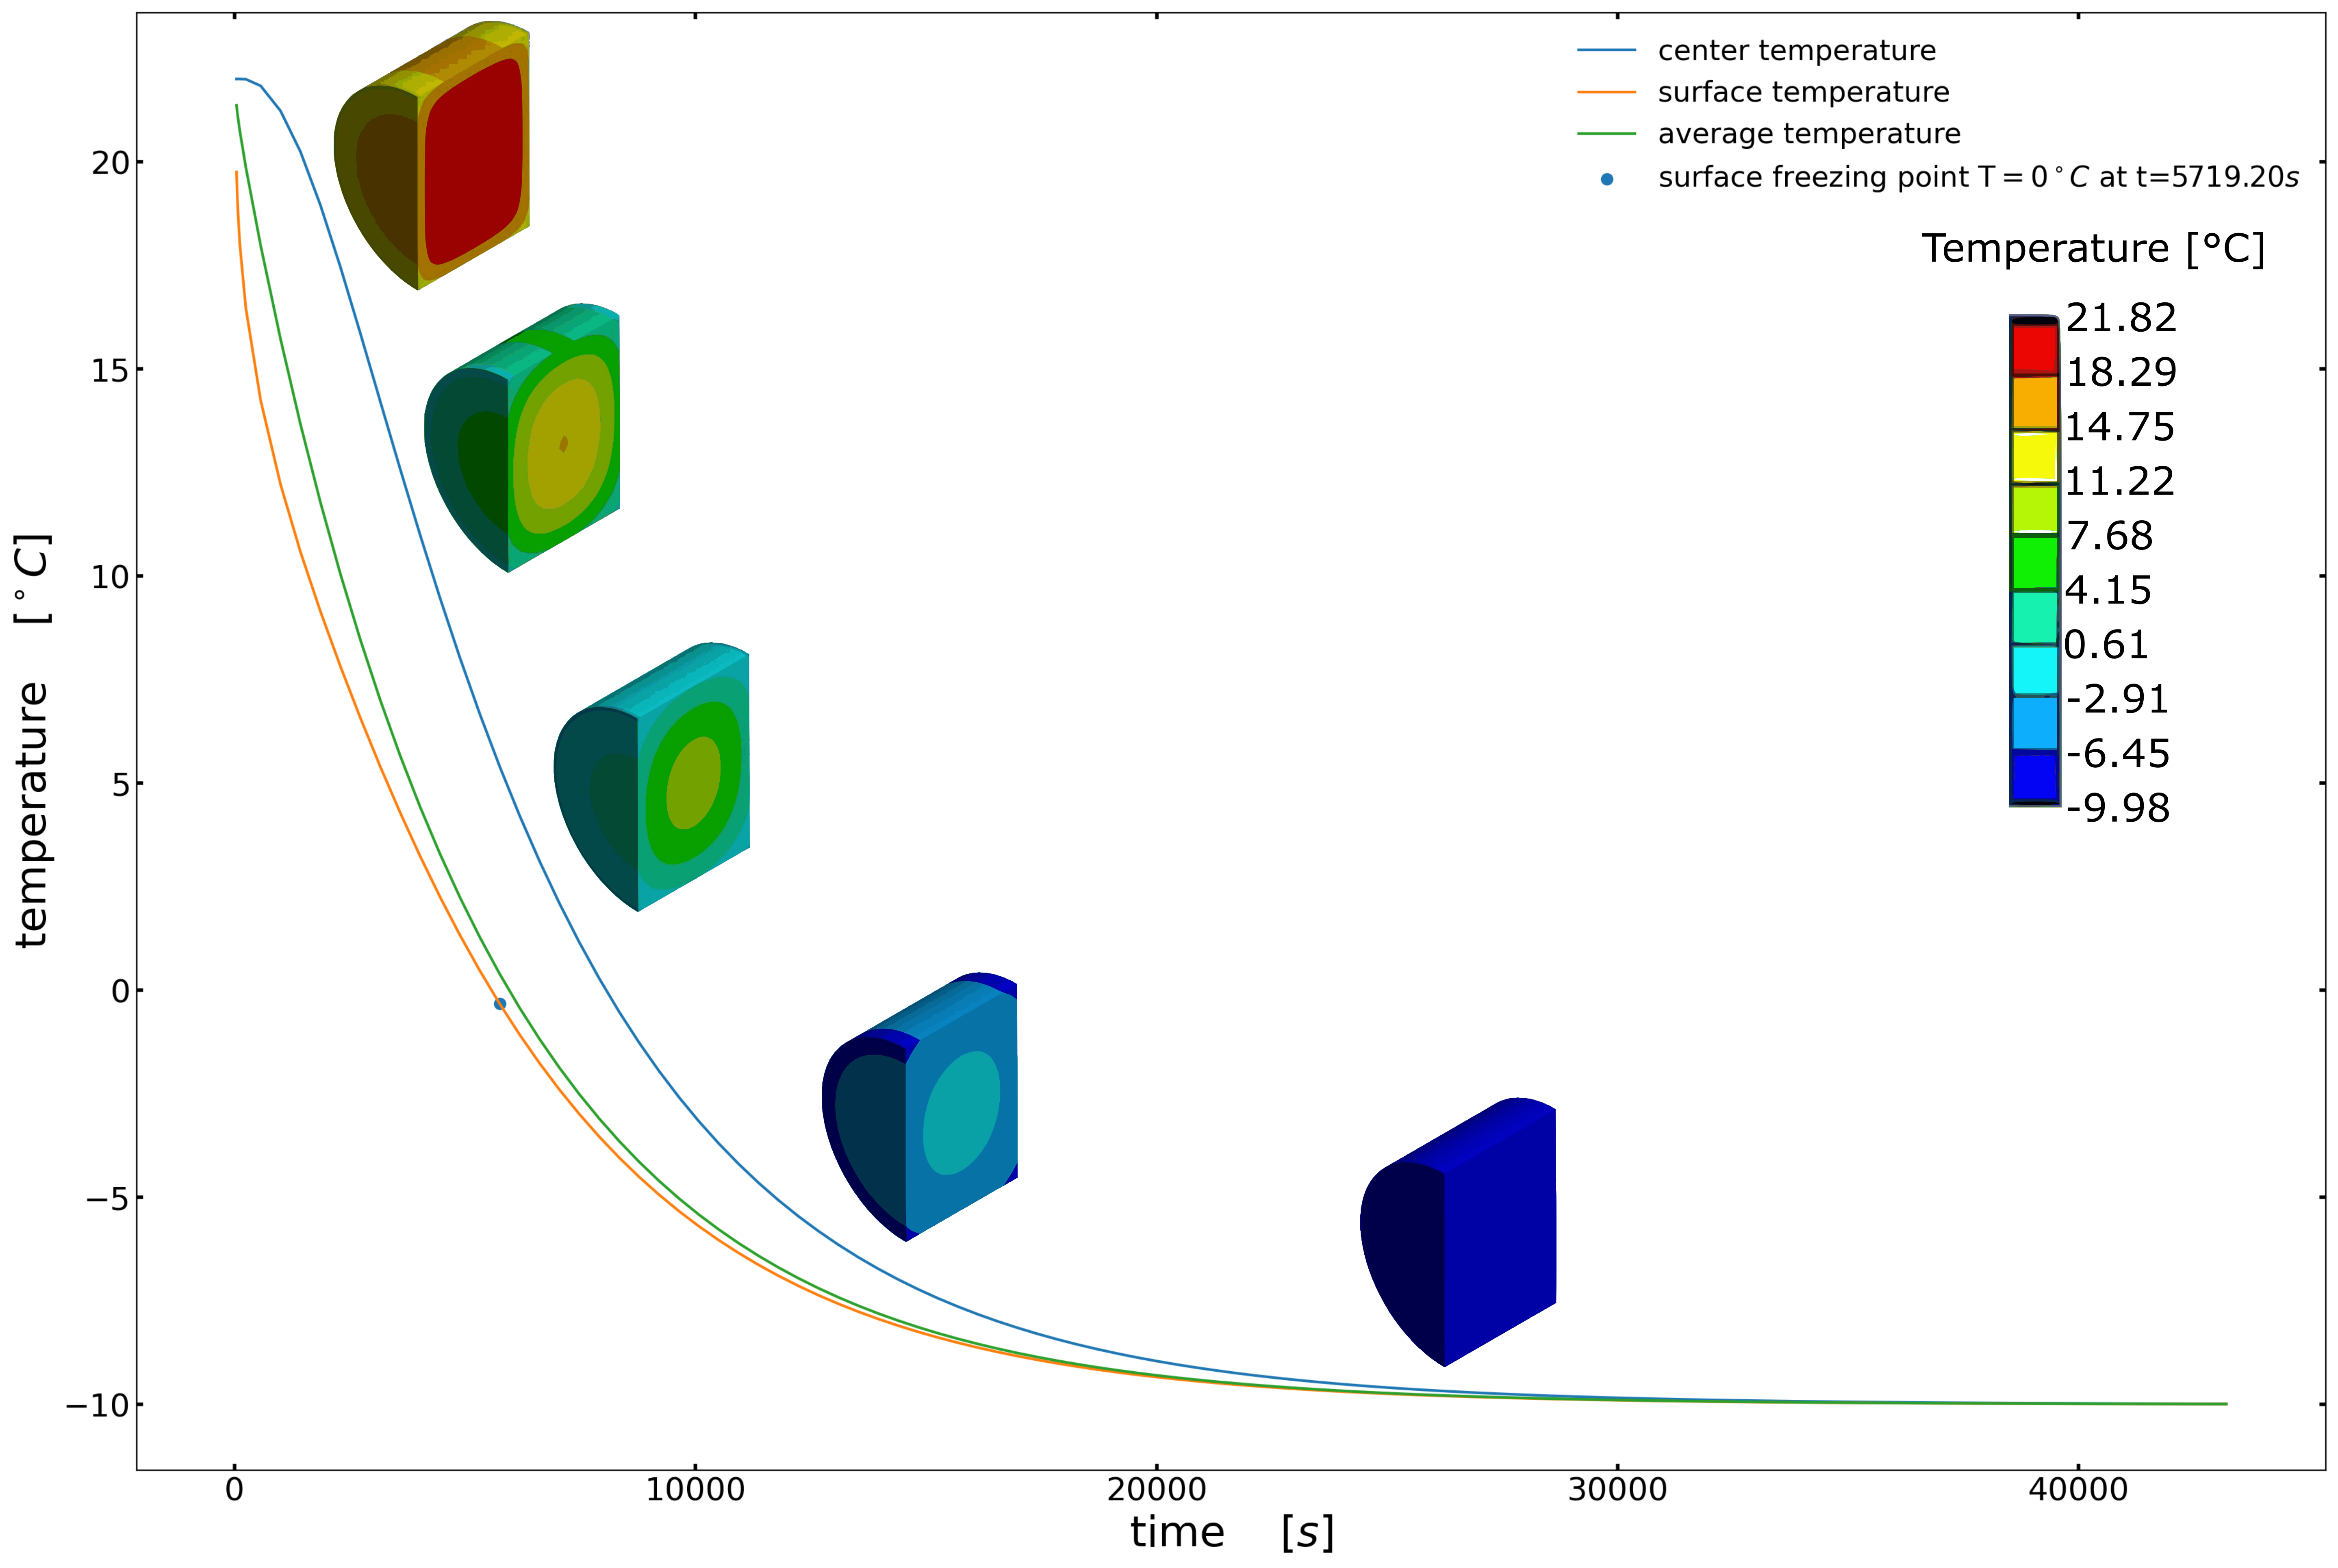
\includegraphics[width=1.00\textwidth]{./cylinderTemps.png}
	\caption{Visualization of a Velocity Field}
	\label{img:cylinderTemps}
\end{figure}

Given the geometry diameter of $5 \textrm{cm}$ given the following:

\begin{dmath}
\rho c_p \frac{\partial T}{\partial t} + \rho c_p v \Lambda T = \nabla \cdot (k \nabla T) + \dot{Q_v}
\end{dmath}

Where: $\displaystyle \rho c_p \frac{\partial T}{\partial t}$ is the accumulation of internal energy, $\displaystyle \rho c_p v \nabla T$ is the convection term, $\displaystyle \nabla \cdot (k \nabla T)$ is the conduction term, and $\displaystyle \dot{Q_v}$ is the metabolic heat reate of the fruit.

With the following boundary conditions at the surface:

\begin{dmath}
\left| k \nabla T + h \right|_{surf} = h (T - T_f) + \varepsilon \sigma (T^4 - {T_w}^4) + \dot{Q_A}
\end{dmath}

\printbibliography[title={References}]
\end{document}
